\documentclass[conference]{IEEEtran}
\IEEEoverridecommandlockouts
% The preceding line is only needed to identify funding in the first footnote. If that is unneeded, please comment it out.
%Template version as of 6/27/2024

\usepackage{cite}
\usepackage{url}
\usepackage{amsmath,amssymb,amsfonts}
\usepackage{algorithmic}
\usepackage{graphicx}
\usepackage{textcomp}
\usepackage{xcolor}
\def\BibTeX{{\rm B\kern-.05em{\sc i\kern-.025em b}\kern-.08em
    T\kern-.1667em\lower.7ex\hbox{E}\kern-.125emX}}
\begin{document}

\title{Depression risk estimation among adults using machine learning models\\
{\footnotesize \textsuperscript{*}Note: Sub-titles are not captured for https://ieeexplore.ieee.org  and
should not be used}
\thanks{Identify applicable funding agency here. If none, delete this.}
}
\author{
\IEEEauthorblockN{1\textsuperscript{st} Caiza}
\IEEEauthorblockA{\textit{Departamento de Ciencias de la} \\
\textit{Computación} \\
\textit{Universidad de las Fuerzas Armadas}\\
\textit{ESPE}\\
Sangolquí, Ecuador \\
cdcaiza5@espe.edu.ec}
\and
\IEEEauthorblockN{2\textsuperscript{nd} Frias}
\IEEEauthorblockA{\textit{Departamento de Ciencias de la} \\
\textit{Computación} \\
\textit{Universidad de las Fuerzas Armadas}\\
\textit{ESPE}\\
Sangolquí, Ecuador \\
pafrias@espe.edu.ec}
\and
\IEEEauthorblockN{3\textsuperscript{rd} Villarroel}
\IEEEauthorblockA{\textit{Departamento de Ciencias de la} \\
\textit{Computación} \\
\textit{Universidad de las Fuerzas Armadas}\\
\textit{ESPE}\\
Sangolquí, Ecuador \\
jjvillarroel1@espe.edu.ec}
}

\maketitle

\begin{abstract}
This document is a model and instructions for \LaTeX.
This and the IEEEtran.cls file define the components of your paper [title, text, heads, etc.]. *CRITICAL: Do Not Use Symbols, Special Characters, Footnotes, 
or Math in Paper Title or Abstract.
\end{abstract}

\begin{IEEEkeywords}
machine learning, depression, predictive modeling, digital biomarkers, BRFSS
\end{IEEEkeywords}

\section{Introduction}

Major depressive disorder represents one of the most critical public health challenges globally, profoundly affecting patients' quality of life and straining healthcare systems. Traditionally, clinical diagnosis and treatment selection have relied heavily on subjective psychiatric evaluations and a reactive, ``trial and error'' paradigm \cite{sokolov_decoding_2024, popescu_evaluating_2021}%[cite: 3]. 
As the global burden of mental health disorders grows, there is an urgent need to transition toward proactive, preventative, and personalized psychiatric care.

In recent years, Artificial Intelligence (AI) has emerged as a transformative tool in psychiatric research and decision-making \cite{chiang_systematic_2025}%[cite: 3]. 
Cutting-edge studies have successfully applied machine learning (ML) and deep learning algorithms to predict depression using complex clinical biomarkers. For instance, predictive models have been trained on high-dimensional gray-matter structures from brain magnetic resonance imaging (MRI) \cite{jiang_applying_2026}%[cite: 3], 
blood DNA methylation profiles \cite{sokolov_decoding_2024}%[cite: 3], 
and multimodal sensing networks that integrate audio, video, and text data \cite{zhang_multimodal_2024}%[cite: 3]. 
Furthermore, AI-powered Clinical Decision Support Systems (CDSS) have been developed to predict psychotherapy remission rates \cite{kannampallil_cross-trial_2022}%[cite: 3], 
demonstrating clinical feasibility and acceptability without negatively impacting the physician-patient relationship during real-world consultations \cite{popescu_evaluating_2021, tanguay-sela_evaluating_2022}%[cite: 3].

Despite these significant technological advances, a notable gap remains in the translational application of these predictive models to routine clinical practice \cite{chiang_systematic_2025}%[cite: 3]. 
Many state-of-the-art diagnostic algorithms depend on expensive, highly specialized, or invasive data sources (e.g., neuroimaging or genomics) that are not readily available in standard primary care or community settings. However, few studies have deeply explored the predictive power of highly accessible, self-reported community health data to proactively estimate depression risk. There remains an unresolved need to evaluate how everyday socio-demographic, economic, and behavioral variables can act as reliable ``digital biomarkers'' on a large population scale.

To address this knowledge gap, this study aims to estimate the risk of depression in adults through a comparative evaluation of robust machine learning classifiers, utilizing everyday health variables and associated risk factors. By transforming static epidemiological data into a dynamic predictive tool, this research seeks to identify which behavioral and psychosocial biomarkers exhibit the strongest predictive influence on depression. Ultimately, the contribution of this work lies in demonstrating the viability of using accessible, non-invasive community data to support early risk detection and personalized psychiatric interventions.

The remainder of this article is organized as follows: Section II details the methodology, including the dataset extraction, feature ranking, and the configuration of the machine learning algorithms. Section III presents the experimental results and performance metrics. Section IV provides a discussion of the clinical implications of the findings. Finally, Section V concludes the paper and outlines future research directions.

\section{Method}

\subsection{Study Approach and Design}
This article develops a predictive and comparative study based on a quantitative and descriptive approach. The primary goal of the research is to estimate the risk of depression in adults through a comparative evaluation of machine learning algorithms, identifying which socio-demographic and behavioral biomarkers exert the greatest predictive influence. A non-experimental, cross-sectional design is proposed, analyzing retrospective epidemiological databases to construct a clinical classification model \cite{sokolov_decoding_2024} %[cite: 3].

\subsection{Development Methodology}
For the execution of the project, the CRISP-DM (Cross-Industry Standard Process for Data Mining) methodology \cite{chapman2000crisp} %[cite: 3] 
was adopted. This framework was chosen due to its cyclical and industry-standard structure, which is ideal for the systematic development of predictive models in the healthcare domain. The analytical tools were based on the Python programming language, utilizing specialized libraries such as Pandas \cite{mckinney2010pandas} %[cite: 3] 
for tabular manipulation via \texttt{pyreadstat} %[cite: 1], 
and Scikit-learn \cite{scikit-learn} %[cite: 3] 
for algorithmic modeling.

\subsection{Data Source and Extraction Methodology}
The analyzed data originate from the \textit{Behavioral Risk Factor Surveillance System} (BRFSS, 2024 cycle) %[cite: 1], 
a large-scale epidemiological surveillance survey conducted by the Centers for Disease Control and Prevention (CDC) \cite{cdc2024brfss} %[cite: 3]. 
The original dataset is massive, containing over $400,000$ records and approximately $300$ individual variables representing a wide array of population health metrics %[cite: 1]. 

To ensure computational efficiency and focus on the most relevant information, data extraction was managed using the \texttt{pyreadstat} library, selectively loading only the required columns directly from the \texttt{.XPT} file %[cite: 1]. 
This extraction methodology prevents memory overload and speeds up the preprocessing pipeline %[cite: 1].

\subsection{Study Variables and Target Definition}

The definitive clinical target variable for this predictive model is \texttt{ADDEPEV3}, which represents whether a patient has ever been told by a health professional that they have a depressive disorder \cite{cdc2024brfss} %[cite: 1, 2, 3]. 
During the data preparation pipeline, this categorical variable is mathematically binarized, mapping positive diagnoses to 1 and negative diagnoses to 0, while strictly discarding non-responses to maintain the integrity of the supervised learning process %[cite: 1]. 
While variables such as \texttt{\_MENT14D} were evaluated, \texttt{ADDEPEV3} was selected as the primary target due to its direct and definitive clinical diagnostic value %[cite: 1, 2].

The BRFSS 2024 dataset inherently contains hundreds of demographic, socioeconomic, and health-related metrics %[cite: 1]. 
To isolate the most relevant socio-behavioral biomarkers and optimize computational efficiency, a Random Forest feature importance algorithm was executed to evaluate and rank the top 30 variables %[cite: 1]. 
These extracted features were categorized into distinct predictive tiers based on their influence scores: \textit{Leakage}, \textit{Strong}, \textit{Moderate}, and \textit{Weak}.

As detailed in Table \ref{tab_rf_importance}, features classified as \textit{Strong} (e.g., \texttt{DECIDE}, \texttt{DIFFALON}, \texttt{LSATISFY}) demonstrate a robust and legitimate predictive relationship with the \texttt{ADDEPEV3} target, representing critical cognitive and psychosocial states. Notably, because a definitive depression diagnosis (\texttt{ADDEPEV3}) is the chosen target, variables measuring recent severe mental health symptoms---such as \texttt{\_MENT14D} (14+ days of poor mental health) and \texttt{MENTHLTH}---act as direct clinical proxies %[cite: 1]. 
Consequently, these are classified as \textit{Leakage} (data leakage) and must be rigorously monitored or excluded during final clinical deployment to prevent artificial inflation of the diagnostic performance metrics.
\begin{table}[htbp]
\caption{Top-30 Biomarkers Ranked by Random Forest Importance}
\begin{center}
\begin{tabular}{|l|p{4.5cm}|c|}
\hline
\textbf{Variable}&\multicolumn{2}{|c|}{\textbf{Attribute Details}} \\
\cline{2-3} 
\textbf{Name} & \textbf{\textit{Brief Description}}& \textbf{\textit{Tier}} \\
\hline
\textit{ADDEPEV3} & Target: Lifetime depression diagnosis. & Strong \\
DECIDE & Difficulty concentrating, remembering, or making decisions & Strong \\

MENTHLTH & Number of days with poor mental health & Leakage$^{\mathrm{a}}$ \\

POORHLTH & Days where poor health limited usual activities & Leakage$^{\mathrm{a}}$ \\

DIFFALON & Difficulty doing errands alone & Strong \\

\_PHYS14D & 14+ days of poor physical health & Leakage$^{\mathrm{a}}$ \\

EMPLOY1 & Current employment status & Moderate \\

GENHLTH & General health self-assessment & Strong \\

SDLONELY & Frequency of feeling lonely or socially isolated & Strong \\

\_AGE80 & Patient's age (imputed, collapsed above 80) & Weak \\

\_RFHLTH & Self-reported good or better general health & Leakage$^{\mathrm{a}}$ \\

\_SEX & Biological gender of the participant & Weak \\

\_BMI5 & Computed Body Mass Index (BMI) & Weak \\

PHYSHLTH & Number of days with poor physical health & Strong \\

\_AGEG5YR & Patient's age, categorized in 5-year ranges & Weak \\

ECIGNOW3 & Current e-cigarette use status & Moderate \\

LSATISFY & Self-reported life satisfaction level & Strong \\

ASTHMA3 & Ever diagnosed with asthma & Strong \\

\_LTASTH1 & Computed lifetime asthma status & Weak \\

\_ASTHMS1 & Computed current asthma status & Weak \\

HEIGHT3 & Reported height & Moderate \\

\_AIDTST4 & Computed indicator for ever being tested for HIV & Weak \\

WTKG3 & Computed weight in kilograms & Weak \\

\_CASTHM1 & Computed current asthma status (alternative) & Weak \\

HAVARTH4 & Ever diagnosed with arthritis & Strong \\

\_DRDXAR2 & Computed diagnosed arthritis status & Weak \\

HIVTST7 & Ever tested for HIV & Moderate \\

HIVTSTD3 & Date or month of last HIV test & Weak \\

WEIGHT2 & Reported weight & Moderate \\

\_AGE\_G & Patient's age categorized into 6 broader levels & Weak \\
\hline
\multicolumn{3}{p{8cm}}{$^{\mathrm{a}}$\textit{Leakage} (Data Leakage) indicates variables that act as direct proxies for the target variable (e.g., self-reporting poor mental health days directly correlates with a depression diagnosis). These are often flagged for exclusion in deployment models to prevent artificial score inflation.}
\end{tabular}
\label{tab_rf_importance}
\end{center}
\end{table}

\subsection{Data Preparation and Processing}
Data cleaning constituted a critical phase to avoid mathematical biases. According to the BRFSS codebook \cite{cdc2024brfss} %[cite: 3], 
specific numerical codes like $7$, $9$, $14$, $77$, and $99$ represent non-responses (e.g., ``Don't know'' or ``Refused'') %[cite: 1]. 
These were mapped to \textit{NaN} to prevent models from interpreting them as continuous weights %[cite: 1]. 
Additionally, values of $88$ in physical and mental health days (meaning ``None'') were explicitly mapped to $0$ to preserve their clinical meaning %[cite: 1].

A cumulative \texttt{ace\_score} was engineered by aggregating binary and frequency responses across 11 Adverse Childhood Experience variables %[cite: 1]. 
Categorical variables were processed using smoothed mean encoding and One-Hot Encoding, while numerical variables were normalized using a Standard Scaler %[cite: 1]. 
Finally, missing values were imputed using the median for numeric/ordinal data and the mode for categorical data %[cite: 1].

\subsection{Dataset Partitioning and Balancing Justification}
Given the highly imbalanced nature of epidemiological datasets (where healthy individuals vastly outnumber those with depression), a 5-fold Stratified Cross-Validation (\texttt{StratifiedKFold}) technique was implemented %[cite: 1]. 
This methodology ensures that the exact proportion of the target class is preserved across all training and validation folds, allowing for robust evaluation %[cite: 1]. 

To handle class imbalance without losing the predictive signal of the minority class, techniques such as Synthetic Minority Over-sampling Technique for Nominal and Continuous data (SMOTENC) and algorithmic class weighting (\texttt{class\_weight}) were employed during the training loops %[cite: 1].

\subsection{Data Modeling and Hyperparameter Justification}
Five machine learning architectures were deployed. The hyperparameters for each algorithm were meticulously configured to optimize predictive capacity while strictly preventing overfitting %[cite: 1]:

\begin{itemize}
    \item \textbf{Random Forest:} Configured with \texttt{n\_estimators=300} to ensure a stable ensemble and restricted to \texttt{max\_depth=12} to prevent the trees from learning noise in the training set. %[cite: 1]
    \item \textbf{LinearSVC:} Wrapped in a \texttt{CalibratedClassifierCV} (with 3-fold cross-validation and sigmoid method) to extract reliable probability estimates (\texttt{predict\_proba}) from the margins. %[cite: 1]
    \item \textbf{Logistic Regression:} Utilized the \texttt{newton-cholesky} solver, which is highly efficient for large, dense datasets. %[cite: 1]
    \item \textbf{XGBoost:} Gradient boosting framework set to \texttt{max\_depth=6} and \texttt{learning\_rate=0.1} to control the complexity of individual trees and avoid gradient explosion. %[cite: 1]
    \item \textbf{LightGBM:} Set to \texttt{n\_estimators=300} and \texttt{learning\_rate=0.1} for rapid, histogram-based boosting. %[cite: 1]
\end{itemize}

All models utilized a fixed random state (\texttt{random\_state=42}) to guarantee the reproducibility of the experiments %[cite: 1].

\subsection{Evaluation Metrics}
Instead of relying solely on baseline accuracy, the models were evaluated using a comprehensive suite of metrics appropriate for imbalanced clinical data, avoiding theoretical mathematical derivations in favor of applied clinical relevance:

\begin{itemize}
    \item \textbf{F1-Score \& Recall:} Recall (Sensitivity) measures the model's ability to identify true depression cases, minimizing dangerous false negatives. The F1-Score provides the harmonic mean between precision and recall, ensuring a balanced performance. %[cite: 1]
    \item \textbf{ROC-AUC \& PR-AUC:} The Area Under the Receiver Operating Characteristic (ROC-AUC) curve evaluates the model's discriminative threshold. Given the class imbalance, the Precision-Recall AUC (PR-AUC) was also calculated to provide a stricter performance penalty for false positives. %[cite: 1]
    \item \textbf{Brier Score \& Confusion Matrix:} The Brier score measures the exactness of the probabilistic outputs, while the accumulated Confusion Matrix provides a direct visualization of true positive, true negative, false positive, and false negative predictions across the 5 folds. %[cite: 1]
\end{itemize}

\subsection{Implementation Environment}
The system was implemented using a high-performance computational environment executed via Python scripts. Mathematical processing relied on NumPy \cite{harris2020array} %[cite: 3] 
and Pandas \cite{mckinney2010pandas} %[cite: 3] 
modules, while the machine learning experimentation framework depended on the Scikit-Learn \cite{scikit-learn} %[cite: 3] 
ecosystem.


\section{Results}

The findings of the predictive modeling experiment are presented based on the evaluation of five machine learning architectures over a 5-fold stratified cross-validation process. The algorithms were evaluated primarily on their ability to detect the \texttt{ADDEPEV3} target using the top 30 socio-behavioral biomarkers.

Table \ref{tab:model_results} summarizes the general statistical performance metrics for each model. The results indicate that the XGBoost algorithm achieved the highest overall Accuracy (0.838) and ROC AUC (0.838), alongside the lowest Brier Score (0.117), which measures the exactness of probabilistic predictions. Linear SVC followed closely in terms of general accuracy (0.834) and demonstrated the highest Specificity (0.951). 

However, when evaluating specific metrics crucial for clinical screening—namely, the ability to correctly identify positive cases of depression—the LightGBM model outperformed all others. LightGBM achieved the highest Recall (Sensitivity) at 0.744, the highest F1-Score (0.579), and the highest Precision-Recall AUC (PR AUC) at 0.628. Random Forest and Logistic Regression presented similar moderate behaviors, both achieving an Accuracy of approximately 0.76 and a Recall above 0.73.

\begin{table}[htbp]
\caption{Model Evaluation Results (Average of 5 iterations)}
\label{tab:model_results}
\centering
\scriptsize
\setlength{\tabcolsep}{3pt}
\renewcommand{\arraystretch}{1.15}
\resizebox{\columnwidth}{!}{
\begin{tabular}{|l|c|c|c|c|c|c|c|c|}
\hline
\textbf{Model} & \textbf{Accuracy} & \textbf{Precision} & \textbf{Recall} & \textbf{F1-Score} & \textbf{Specificity} & \textbf{ROC AUC} & \textbf{PR AUC} & \textbf{Brier Score} \\
\hline
Random Forest & 0.766 & 0.467 & 0.743 & 0.573 & 0.772 & 0.834 & 0.619 & 0.160 \\
\hline
Linear SVC & 0.834 & 0.688 & 0.399 & 0.505 & 0.951 & 0.832 & 0.614 & 0.119 \\
\hline
Logistic Regression & 0.769 & 0.471 & 0.732 & 0.573 & 0.780 & 0.833 & 0.615 & 0.162 \\
\hline
XGBoost & \textbf{0.838} & 0.687 & 0.428 & 0.528 & 0.947 & \textbf{0.838} & 0.627 & \textbf{0.117} \\
\hline
LightGBM & 0.771 & 0.474 & \textbf{0.744} & \textbf{0.579} & 0.779 & \textbf{0.838} & \textbf{0.628} & 0.158 \\
\hline
\end{tabular}
}
\end{table}

The accumulated confusion matrices detail the specific classification behavior across the evaluated folds. As observed in Figure \ref{fig:cm_lightgbm}, LightGBM successfully identified 71,599 true positive cases of depression, significantly minimizing false negatives (24,526). In contrast, while XGBoost (Figure \ref{fig:cm_xgboost}) and Linear SVC excelled at identifying true negatives (340,167 and 341,474 respectively), they incurred a severe clinical cost by missing a large volume of actual depression cases, registering 54,923 and 57,721 false negatives, respectively.

\begin{figure}[htbp]
\centering
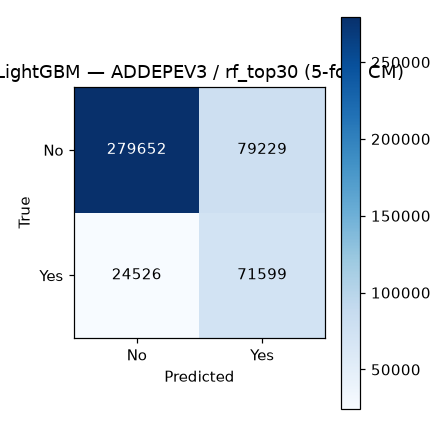
\includegraphics[width=0.35\textwidth]{Imagenes/cm_LightGBM_ADDEPEV3_rf_top30_class_weight.png}
\caption{Confusion Matrix for LightGBM (5-fold Cross-Validation)}
\label{fig:cm_lightgbm}
\end{figure}

\begin{figure}[htbp]
\centering
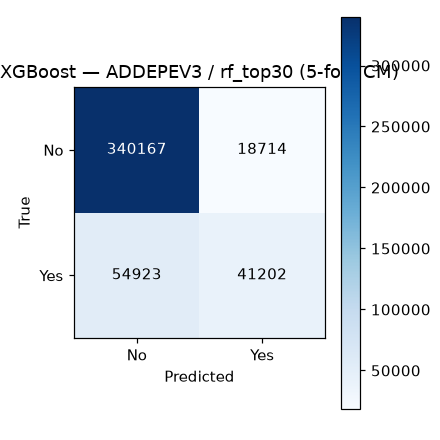
\includegraphics[width=0.35\textwidth]{Imagenes/cm_XGBoost_ADDEPEV3_rf_top30_class_weight.png}
\caption{Confusion Matrix for XGBoost (5-fold Cross-Validation)}
\label{fig:cm_xgboost}
\end{figure}

\section{Discussion}

The primary objective of this study was to estimate the risk of depression in adults by identifying the most influential socio-behavioral biomarkers and evaluating various predictive algorithms. The results indicate that gradient boosting frameworks—specifically LightGBM and XGBoost—are highly effective at modeling complex, non-linear epidemiological data, surpassing traditional linear approaches. 

A critical finding of this research is the pronounced clinical trade-off between general Accuracy and Sensitivity (Recall). While XGBoost achieved the highest theoretical Accuracy (0.838), it did so by favoring the majority class (healthy individuals), resulting in a poor Recall of 0.428. In the context of public health and psychiatric screening, prioritizing Specificity over Sensitivity is dangerous, as it leaves highly vulnerable adults undetected. Therefore, LightGBM emerges as the most clinically relevant model; its superior Recall (0.744) and PR AUC (0.628) prove its capacity to capture the underlying patterns of depression risk, minimizing false negatives. This superiority can be explained by LightGBM's leaf-wise tree growth strategy, which handles imbalanced, high-dimensional categorical data more efficiently than depth-wise algorithms.

Despite these promising results, the study presents methodological limitations. The reliance on the BRFSS dataset implies that the input variables are self-reported, making them susceptible to recall bias and subjective underreporting of symptoms. Furthermore, while class weighting techniques were applied, the Precision across all models remained relatively low (e.g., LightGBM Precision = 0.474). This indicates a high rate of false positives, an inherent challenge when working with highly imbalanced epidemiological data where symptoms overlap with other conditions.

Future research should focus on mitigating these false positives through more advanced resampling techniques or ensemble methods. Additionally, future works should evaluate the \texttt{\_MENT14D} variable (recent poor mental health days) as a primary target to transition from predicting lifetime diagnoses to predicting acute, real-time depressive episodes.

\section{Conclusions}

This study successfully demonstrated that machine learning algorithms can reliably estimate the risk of lifetime depression in adults utilizing accessible, non-invasive behavioral and psychosocial data. By identifying key digital biomarkers, this research confirms that everyday variables—such as socioeconomic status, adverse childhood experiences, and physical health metrics—hold substantial predictive power, reducing the reliance on costly clinical tests.

Among the evaluated architectures, LightGBM proved to be the most viable model for psychiatric screening. By achieving the highest Recall (0.744) and F1-Score (0.579), it effectively minimized the misclassification of vulnerable patients, addressing the core objective of prioritizing early and accurate risk detection. 

The developed predictive framework offers direct practical applications for healthcare systems. These models can be seamlessly integrated into Clinical Decision Support Systems (CDSS) within primary care settings to automatically flag at-risk individuals using standard patient intake forms. Future investigations should expand the feature set and focus on longitudinal validations to further refine the precision of the algorithm in diverse clinical environments.
\bibliographystyle{ieeetr} 
\bibliography{Principal_Data} 

\vspace{12pt}
\end{document}